%%%%%%%%%%%%%%%%%%%%%%%%%%%%%%%%%%%%%%%%%
% Beamer Presentation
% LaTeX Template
% Version 1.0 (10/11/12)
%
% This template has been downloaded from:
% http://www.LaTeXTemplates.com
%
% License:
% CC BY-NC-SA 3.0 (http://creativecommons.org/licenses/by-nc-sa/3.0/)
%
%%%%%%%%%%%%%%%%%%%%%%%%%%%%%%%%%%%%%%%%%

%----------------------------------------------------------------------------------------
%	PACKAGES AND THEMES
%----------------------------------------------------------------------------------------

\documentclass{beamer}

\mode<presentation> {

% The Beamer class comes with a number of default slide themes
% which change the colors and layouts of slides. Below this is a list
% of all the themes, uncomment each in turn to see what they look like.

%\usetheme{default}
%\usetheme{AnnArbor}
%\usetheme{Antibes}
%\usetheme{Bergen}
%\usetheme{Berkeley}
%\usetheme{Berlin}
%\usetheme{Boadilla}
%\usetheme{CambridgeUS}
%\usetheme{Copenhagen}
%\usetheme{Darmstadt}
%\usetheme{Dresden}
%\usetheme{Frankfurt}
%\usetheme{Goettingen}
%\usetheme{Hannover}
%\usetheme{Ilmenau}
%\usetheme{JuanLesPins}
%\usetheme{Luebeck}
\usetheme{Madrid}
%\usetheme{Malmoe}
%\usetheme{Marburg}
%\usetheme{Montpellier}
%\usetheme{PaloAlto}
%\usetheme{Pittsburgh}
%\usetheme{Rochester}
%\usetheme{Singapore}
%\usetheme{Szeged}
%\usetheme{Warsaw}

% As well as themes, the Beamer class has a number of color themes
% for any slide theme. Uncomment each of these in turn to see how it
% changes the colors of your current slide theme.

%\usecolortheme{albatross}
%\usecolortheme{beaver}
%\usecolortheme{beetle}
%\usecolortheme{crane}
%\usecolortheme{dolphin}
%\usecolortheme{dove}
%\usecolortheme{fly}
%\usecolortheme{lily}
%\usecolortheme{orchid}
%\usecolortheme{rose}
%\usecolortheme{seagull}
\usecolortheme{seahorse}
%\usecolortheme{whale}
%\usecolortheme{wolverine}

\setbeamertemplate{footline} % To remove the footer line in all slides uncomment this line
%\setbeamertemplate{footline}[page number] % To replace the footer line in all slides with a simple slide count uncomment this line

\setbeamertemplate{navigation symbols}{} % To remove the navigation symbols from the bottom of all slides uncomment this line
}

\usepackage{graphicx} % Allows including images
\usepackage{ulem} % Allows including images
\usepackage{xcolor} % Allows including images

\let\oldfootnotesize\footnotesize
\renewcommand*{\footnotesize}{\oldfootnotesize\tiny}

\newcommand{\tm}{\mathrm{time}}

\newcommand\rem{\bgroup\markoverwith{\textcolor{red}{\rule[.3ex]{2pt}{1.5pt}}}\ULon}

\title{Fully Polynomial Parameterized Algorithms\\For the \texorpdfstring{$T$}{T}-Path Packing Problem} % The short title appears at the bottom of every slide, the full title is only on the title page

\author{Narek Bojikian} % Your name
\institute[Hu-Berlin]
{
	Humboldt University of Berlin
}
\date{12.12.2019} % Date, can be changed to a custom date

\begin{document}

\begin{frame}
\titlepage % Print the title page as the first slide
\end{frame}

\begin{frame}[t]{Introduction}
	\begin{columns}
		\begin{column}{.5\textwidth}
			\begin{itemize}[<+->]
				\uncover<1->{\item $T$-path packing.}
				\uncover<3->{\item Odd $T$-path packing.}
				\uncover<5->{\item $S-T$-path packing.}
				\uncover<7->{\item[--] Goal: Find maximum set of each.}
				\uncover<9->{\item Maximum Matching - $\nu(G)$.}
			\end{itemize}
		\end{column}
		\begin{column}[c]{.5\textwidth}
			\centering
			\vspace{2cm}
			\only<1>{\makebox[\textwidth][c]{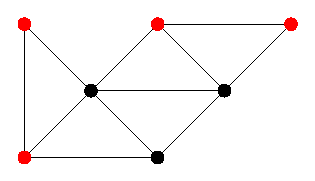
\includegraphics{figures/t-graph.eps}}}
			\only<2>{\makebox[\textwidth][c]{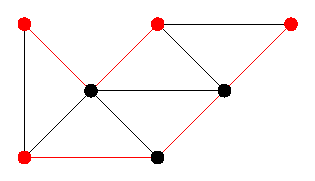
\includegraphics{figures/t-path.eps}}}
			\only<3>{\makebox[\textwidth][c]{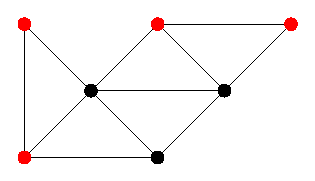
\includegraphics{figures/t-graph.eps}}}
			\only<4>{\makebox[\textwidth][c]{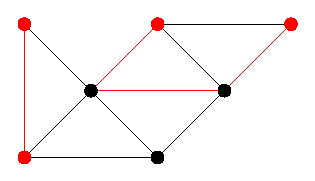
\includegraphics{figures/odd-t-path.eps}}}
			\only<5>{\makebox[\textwidth][c]{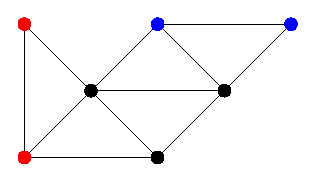
\includegraphics{figures/st-graph.eps}}}
			\only<6-7>{\makebox[\textwidth][c]{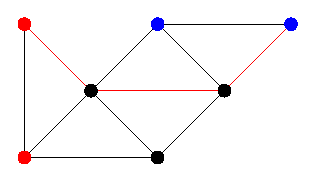
\includegraphics{figures/st-path.eps}}}
			\only<8>{\makebox[\textwidth][c]{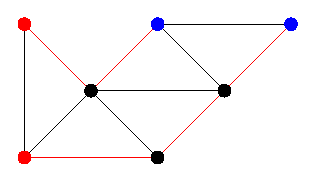
\includegraphics{figures/st-optimal.eps}}}
			\only<9>{\makebox[\textwidth][c]{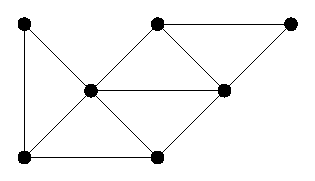
\includegraphics{figures/graph.eps}}}
			\only<10>{\makebox[\textwidth][c]{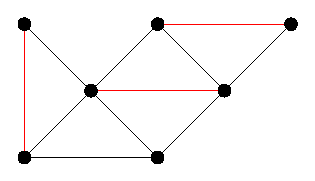
\includegraphics{figures/matching.eps}}}
		\end{column}
	\end{columns}
\end{frame}

\begin{frame}[t]{Reduction - $T$-Path Packing to Matching}
	\begin{minipage}[t][.4\textheight][t]{\linewidth}
		\centering
		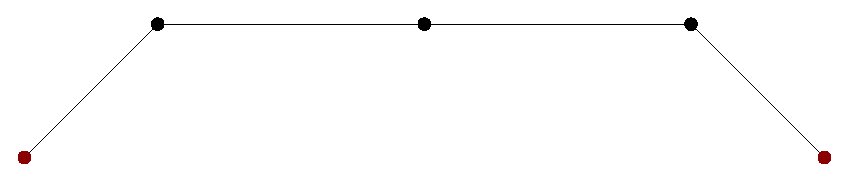
\includegraphics[width=.5\textwidth]{figures/reductions/graph-orig.eps}
	\end{minipage}
	\hfill
	\begin{minipage}[t][.4\textheight][t]{\linewidth}
		\centering
		\uncover<2->{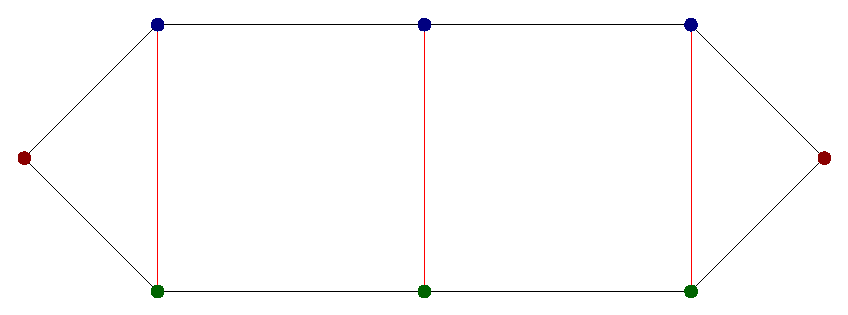
\includegraphics[width=.5\textwidth]{figures/reductions/graph-first.eps}}
	\end{minipage}
	\hrule
	{\tiny Maximum-minimum S{\"a}tze {\"u}ber Graphen, T.Gallai, 1958}
\end{frame}

\begin{frame}{Reductions presented in the thesis}
	\begin{minipage}[t][.3\textheight][t]{\linewidth}
		\begin{minipage}[t][\textheight][t]{.45\linewidth}
		\centering
		\vspace{1cm}
		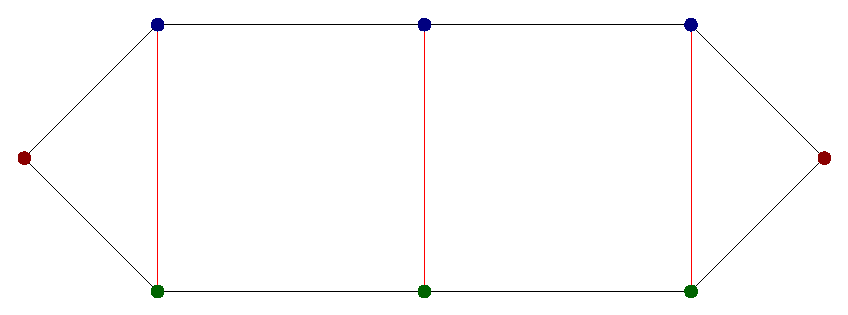
\includegraphics[width=.5\textwidth]{figures/reductions/graph-first.eps}
		
		\centering $T$-Path Packing Problem
		\end{minipage}
		\hfill
		\vline
		\hfill
		\begin{minipage}[t][\textheight][t]{.45\linewidth}
		\centering
		\vspace{1cm}
		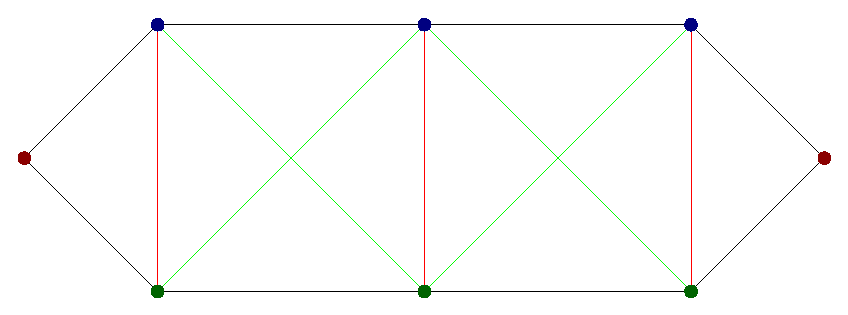
\includegraphics[width=.5\textwidth]{figures/reductions/graph-second.eps}

		\centering $T$-Path Packing Problem
		\end{minipage}
	\end{minipage}
		\vfill
		\hrule
		\vfill
	\begin{minipage}[t][.3\textheight][t]{\linewidth}
		\begin{minipage}[t][\textheight][t]{.45\linewidth}
		\centering
		\vspace{1cm}
		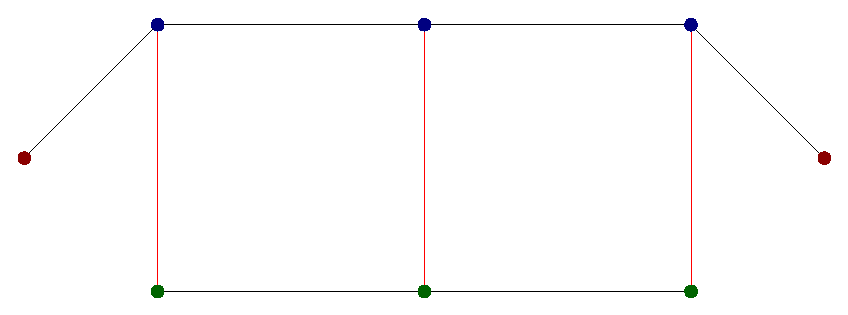
\includegraphics[width=.5\textwidth]{figures/reductions/graph-odd.eps}

		\centering Odd $T$-Path Packing Problem
		\end{minipage}
		\hfill
		\hfill
		\begin{minipage}[t][\textheight][t]{.45\linewidth}
		\centering
		\vspace{1cm}
		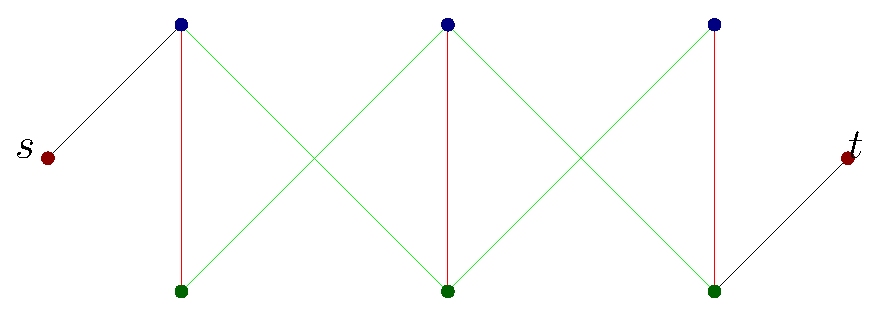
\includegraphics[width=.5\textwidth]{figures/reductions/graph-st.eps}

		\centering $S-T$-Path Packing Problem
		\end{minipage}
	\end{minipage}

\end{frame}

\begin{frame}[t]{Methods and results - Preserving properties}
	\begin{itemize}[<+->]
		\item Let $\mathcal{A}$ be an efficient \textbf{polynomial-time}$^{(*)}$ algorithm for matching in a class $\mathcal{C}$.
		\item Let $f$ be a reduction from a problem $P$ to maximum matching.
		\item Assume $f$ can be computed efficiently and the size of the output is bounded in a \textbf{linear function}$^{(**)}$ in the size of $G$.
		\item Assume $\mathcal{C}$ is closed under $f$.\\
			\uncover<5->{\hspace{.5cm} - Then we get an efficient algorithm for $P$ in $\mathcal{C}$.}
	\end{itemize}

	\vspace{1cm}

	\uncover<6->{
	\begin{block}{$A'$ - Efficient algorithm for $P$}
		Given a graph $G$. Compute $G' := f(G)$ and apply $\mathcal{A}$ on $G'$.
	\end{block}}

	\uncover<7->{$$\tm_{A'}(G) = \tm_f(G) + \tm_A(G') \underset{(*,**)}{=} O(\tm_f(G) + \tm_A(G))$$}

\end{frame}
\begin{frame}[t]{Methods and results - Preserving properties}
\vspace{.5cm}
	\begin{itemize}
		\item $T$-path packing (using the second reduction):
		\begin{itemize}
			\item[--] Tree-depth.
			\item[--] Tree-width.
			\item[--] $s$-plexes.\\ \hspace{.5cm} The value at most doubles.
			\item[--] Modular-width.
			\item[--] Independence number.
			\item[--] Neighborhood diversity number.\\ \hspace{.5cm} The value does not change.\\
				\hspace{5cm} \textcolor{blue}{ .. Running time $O(k(n+m))$}
			\item[--] Strongly chordal -, Interval- and co-Comparability- graphs.\\
				\hspace{.5cm} The classes are closed under this reduction.\\
				\hspace{5cm} \textcolor{blue}{ .. Running time $O(n+m)$}
			\item[--] Circular-arc graphs.\\
				\hspace{.5cm} The classes are closed under this reduction.\\
				\hspace{5cm} \textcolor{blue}{ .. Running time $O((n+m)\log(n))$}
		\end{itemize}
	\end{itemize}
	\hrule
	{\tiny For $n$ the number of the vertices and $m$ the number edges in the graph $G$.}
\end{frame}

\begin{frame}[t]{Methods and results - Preserving properties}
\vspace{.5cm}
	\begin{itemize}
		\item Odd $T$-path packing:
			\begin{itemize}
				\item[--] Neighborhood diversity number.\\
					\hspace{.5cm} - Bounded Replaceablity $O(k^2)$.\\
				\hspace{5cm} \textcolor{blue}{ .. Running time $O(k^2(n+m))$}
			\end{itemize}
		\item Odd $T$-path packing and $S-T$-path packing:
			\begin{itemize}
				\item[--] Tree-depth and tree-width.\\ \hspace{.5cm} The value at most doubles.\\
				\hspace{5cm} \textcolor{blue}{ .. Running time $O(k(n+m))$}
				\item[--] \rem{Independence number - does not change.}
			\end{itemize}
	\end{itemize}
\end{frame}

\begin{frame}[t]{Methods and results - Distance to triviality}
\vspace{.5cm}
\begin{itemize}
	\uncover<1->{\item Vertex-deletion distance to a class - $d_{\mathcal{\mathcal{C}}}(G)$.}


	\uncover<2->{\item The reductions preserve the distance to triviality.\\}
		\uncover<3->{Given a graph $G$, a class $\mathcal{C}$ and any of the reductions $f$ such that\\
		\hspace{.5cm} $\mathcal{C}$ is closed under $f$ and $d_{\mathcal{C}}(G) \leq k$, then
	\hspace{.5cm} \textcolor{blue}{$d_{\mathcal{C}}(f(G)) \leq 2k$}.}

	\uncover<4->{\item The reductions preserve the distance to parameters values.\\}
		\uncover<5->{Let $\rho_G$ be the value of the parameter in $G$. Consider the class $\mathcal{C}_n := \{G : \rho_G \leq n\}$. For a reduction $f$, such that $f(C_n) \subseteq C_{g(n)}$ for some computeable function $g$,\\
	\hspace{.5cm} we get \textcolor{blue}{$d_{\mathcal{C}_{g(n)}}(f(G)) \leq 2d_{C_n}(G)$}.}
	\uncover<6->{\item If maximum matching can be solved efficiently in graphs with distance at most $k$ to $\mathcal{C}$, so is $T$-path packing.}
	\end{itemize}
\end{frame}

\begin{frame}[t]{Methods and results - Distance to triviality}
\vspace{.5cm}
\begin{itemize}
	\uncover<1->{\item $T$-Path Packing.
		\begin{itemize}
			\item[--] Neighborhood diversity number.
			\item[--] $s$-plexes.
			\item[--] Independence number.\\
				\hspace{5cm} \textcolor{blue}{ .. Running time $O(\sqrt{d}k(n+m))$}
		\end{itemize} }
	\uncover<2->{\item Odd $T$-Path Packing.\\
		Neighborhood diversity number.
		\begin{itemize}
			\uncover<3->{\item[--] The class of $\ell$-Replaceable graphs - $\mathcal{R}[\ell]$.}
			\uncover<4->{\item[--] For $m := |E(G)|$, $l, d \in \mathbb{N}$,  if $d_{\mathcal{R}[\ell]}(G) \leq d$,\\
				\hspace{.5cm} then $\nu(G)$ can be found in $O(\sqrt{d}\ell m)$
				\footnote{On adaptive algorithms for maximum matching, F.Hegerefeld and S.Kratsch, ICALP-2019.}.}
			\uncover<5->{\item[--] For $G'$ the graph resulting from $G$ when we apply the second reduction.\\
			If the Neighborhood diversity number of $G$ is at most $k$ then $G'$ is at most $O(k^2)$ replaceable.\\}
			\uncover<6->{\hspace{5cm} \textcolor{blue}{ .. Running time $O(\sqrt{d}k^2(n+m))$}}
		\end{itemize}
	}
\end{itemize}
\end{frame}

\begin{frame}[t]{Methods and results - Simplify, solve and augment}
	\begin{itemize}[<+->]
		\item Sometimes parameters can be seen from\\
			\hspace{.5cm} a different perspective.
		\item[--] The feedback vertex number of a graph\\
			\hspace{.5cm} is the size of the smallest set of vertices\\
			\hspace{.5cm} that intersects all cycles in the graph.
		\item Equivalently, the feedback vertex number of a graph $G$\\
			\hspace{.5cm} is the vertex-deletion distance of this graph\\
			\hspace{.5cm} from forests\footnote{For $\mathcal{T}$ the class of forests.} - $d_{\mathcal{T}}(G)$.
		\item Let $\rho$ be a parameter defined as \\ \hspace{.5cm} - the vertex-deletion distance to a class $\mathcal{C}$.
		\item Assume $T$-Path Packing admits an efficient algorithm $\mathcal{A}$ in $\mathcal{C}$.\\ \hspace{.5cm} - Then we get an algorithm for $G$ parameterized by $\rho$.
	\end{itemize}
\end{frame}

\begin{frame}[t]{Methods and results - Simplify, solve and augment}
	\begin{block}{A' - Parameterized algorithm}
		\begin{itemize}[<+->]
			\item Let $S$ be a modulator in $G$ and $H := G \setminus S$, i.e. $H \in \mathcal{C}$.
			\item Apply $\mathcal{A}$ on $H$.
			\item Apply the first reduction on $H$ to get $H'$.\\
			\item Find a maximum matching in $H$ (using the reduction).
			\item Turn $H$ into $G$ by adding $S$ back to the graph\\
				\hspace{.5cm} - turns $H'$ into $G'$ by adding at most $2|S|$ vertices.
			\item Find a maximum matching in $G'$\\
				\hspace{.5cm} - by finding at most $2|S|$ augmenting paths.
			\item Find a maximum $T$-path packing in $G$ (using the reduction).
		\end{itemize}
	\end{block}
	\vspace{-.5cm}
	\uncover<8->{
	\begin{align*}
		\tm_{A'}(G) &= O(n+m + \tm_{A}(H) + (2|S|(n+m)))\\
		&= O(\tm_{A}(G \setminus S) + \rho(n+m)).
	\end{align*}
	\hrule
	{\tiny For $n$ the number of the vertices and $m$ the number edges in the graph $G$.}
}
\end{frame}

\begin{frame}[t]{Methods and results - Simplify, solve and augment}
\vspace{.5cm}
	\begin{itemize}
		\item Vertex Cover Number\\ \hspace{.5cm} - simplify to an independent set.\\
			{
				
				\hspace{3cm}Running time \textcolor{blue}{ $O(k(n+m))$}$\rightarrow$\textcolor{green}{$O(\sqrt k (n+m)$}\footnote{suggested by Prof. Kratsch.}
			}
		\item Feedback Vertex Number\\ \hspace{.5cm} - simplify to a forest.\\
				\hspace{5cm} \textcolor{blue}{ .. Running time $O(k(n+m))$}
	\end{itemize}
	Designed a dynamic programming algorithm for each of the problems in forests.
\end{frame}

\end{document}
